\section{Stylized facts and correlation structure}
\label{sec:stylized_correlation}

\subsection{Stylized facts of selected B3 assets}

The first empirical figure introduces the behaviour of PETR4, VALE3 and BBDC4. These assets are not used as a miniature market index. They are used because they provide a compact visual entry point into the Brazilian data: a state-linked oil company, a global mining company and a large private bank. Figure~\ref{fig:stylized_facts} combines four diagnostics that are standard in econophysics: normalized prices, daily returns, the complementary cumulative distribution of absolute returns and the autocorrelation of absolute returns.

\begin{figure}
\centering
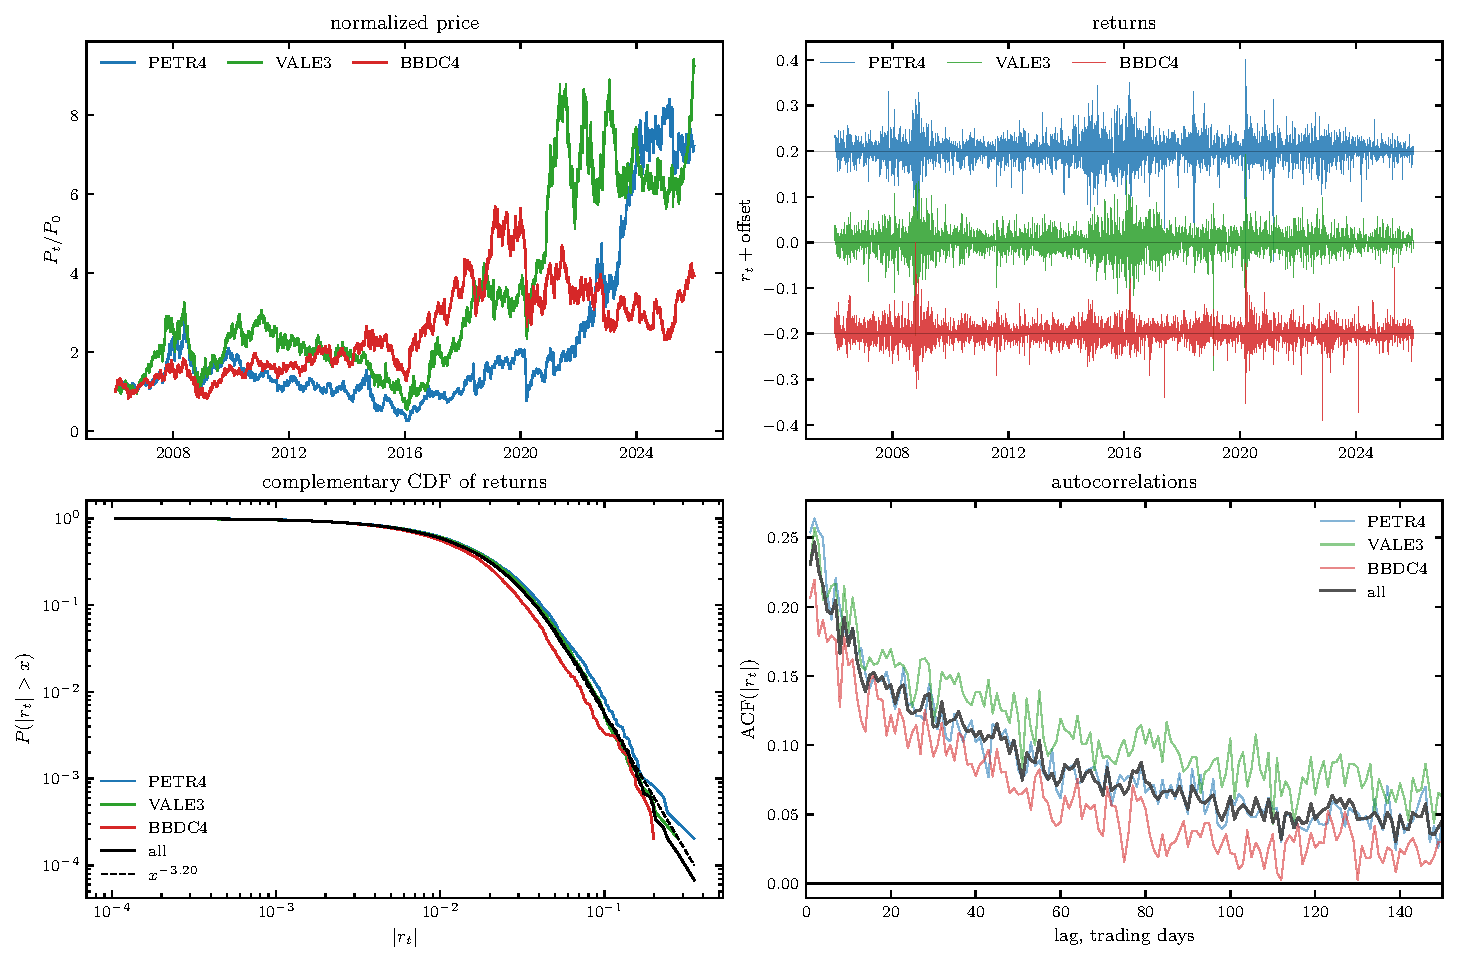
\includegraphics[width=\linewidth]{images/figure_1d_stylized_facts_demo_assets_clean_2006_2025.pdf}
\caption{Stylized facts for PETR4, VALE3 and BBDC4 over 2006--2025. The panels show normalized prices, vertically offset daily log returns, the complementary cumulative distribution of absolute returns and autocorrelations of absolute returns.}
\label{fig:stylized_facts}
\end{figure}
\FloatBarrier

The normalized-price panel shows that even a small set of liquid Brazilian assets contains heterogeneous long-run trajectories. VALE3 reflects commodity and exchange-rate cycles, PETR4 reflects oil prices and political/institutional shocks, and BBDC4 reflects financial-sector dynamics. The return panel shows volatility clustering: large shocks are not isolated uniformly through time but concentrate around stress periods. The CCDF panel shows that large absolute returns are more frequent than a Gaussian benchmark would suggest, confirming the heavy-tailed nature of B3 returns. Finally, the autocorrelation panel shows persistence in $|r_t|$, which is the empirical reason why GARCH(1,1) and HAR-RV later serve as demanding benchmarks for any volatility forecasting model.

\subsection{Descriptive statistics}

Table~\ref{tab:descriptive_stats} quantifies the same diagnostics. All three series have means close to zero, substantial kurtosis and non-negligible counts of large absolute returns. PETR4 has the largest negative daily observation in the 2006--2025 window, while VALE3 and BBDC4 also show stress-period extremes. The autocorrelations of absolute returns remain positive across several lags, especially for VALE3.

\begin{table}
\centering
\caption{Descriptive statistics for the three demonstration assets, 2006--2025.}
\label{tab:descriptive_stats}
\resizebox{\linewidth}{!}{%
\begin{tabular}{lrrrrrrrrrrrrrrr}
\toprule
symbol & $n_{\mathrm{obs}}$ & mean & std & skewness & excess kurtosis & min & max & VaR 1\% & VaR 5\% & $|r|>10\%$ & $|r|>20\%$ & ACF$_1$ & ACF$_5$ & ACF$_{20}$ & ACF$_{60}$ \\
\midrule
BBDC4 & 4953 & 0.00028 & 0.02180 & 0.02 & 7.96 & -0.1910 & 0.1999 & -0.0559 & -0.0312 & 16 & 0 & 0.207 & 0.174 & 0.122 & 0.044 \\
PETR4 & 4953 & 0.00041 & 0.02755 & -0.76 & 11.55 & -0.3524 & 0.2007 & -0.0767 & -0.0408 & 41 & 4 & 0.254 & 0.209 & 0.140 & 0.062 \\
VALE3 & 4953 & 0.00045 & 0.02576 & -0.22 & 7.51 & -0.2814 & 0.1936 & -0.0676 & -0.0381 & 26 & 2 & 0.231 & 0.207 & 0.169 & 0.119 \\
\bottomrule
\end{tabular}}
\end{table}
\FloatBarrier

The descriptive statistics support the visual reading of Figure~\ref{fig:stylized_facts}. The distributions are not symmetric Gaussian series with weak memory in volatility. They show heavy tails and persistent volatility. This justifies treating the Brazilian market as a complex empirical system rather than as a set of independent, homoskedastic return series.

\subsection{Static correlation distribution}

The next step moves from univariate behaviour to cross-sectional dependence. The core historical universe contains 58 assets, producing $N(N-1)/2=1653$ unique asset pairs. Figure~\ref{fig:correlation_structure} summarizes the full pairwise correlation distribution and then splits pairs into within-sector and between-sector groups.

\begin{figure}
\centering
\begin{subfigure}{0.49\linewidth}
  \centering
  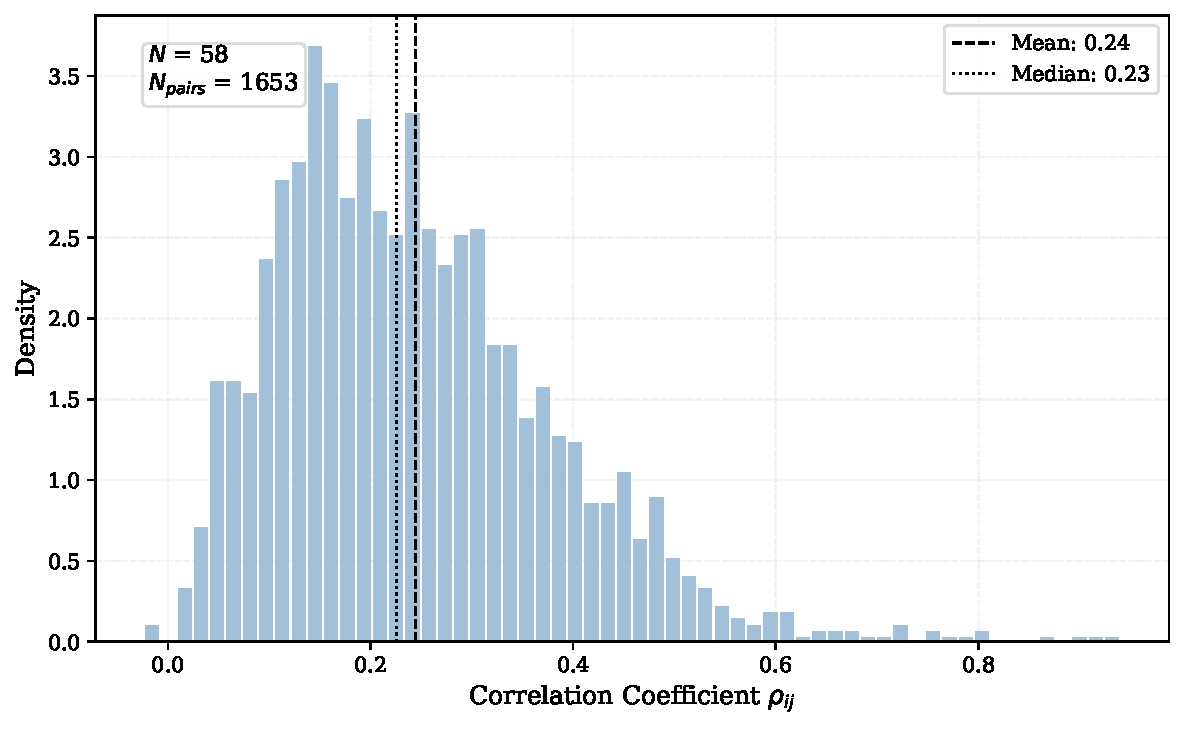
\includegraphics[width=\linewidth]{images/figure_2_correlation_histogram.pdf}
  \caption{Full pairwise distribution.}
  \label{fig:corr_hist}
\end{subfigure}
\hfill
\begin{subfigure}{0.49\linewidth}
  \centering
  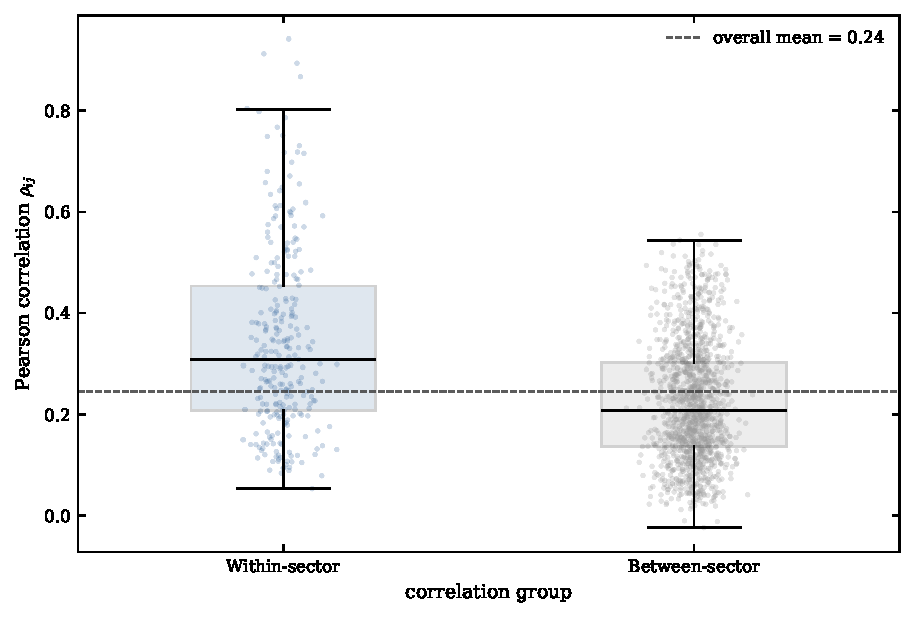
\includegraphics[width=\linewidth]{images/figure_3_sector_correlation_distribution.pdf}
  \caption{Within-sector and between-sector pairs.}
  \label{fig:sector_corr}
\end{subfigure}
\caption{Correlation structure in the core historical universe. Panel (a) shows the full Pearson correlation distribution. Panel (b) compares within-sector and between-sector correlations using the initial macro-sector classification.}
\label{fig:correlation_structure}
\end{figure}
\FloatBarrier

The full distribution is centred in a moderate positive range, with mean correlation close to 0.24 and median correlation close to 0.23. This level of average dependence is large enough to imply a strong common component, but the distribution remains dispersed. The dispersion is important because it leaves room for sectoral and subsectoral organization rather than a single homogeneous market block.

\subsection{Sectoral correlation comparison}

The sector split strengthens this interpretation. Within-sector correlations are visibly shifted to the right relative to between-sector correlations. This is the first direct evidence that the initial macro-sector map is reflected in the empirical dependency matrix.

\begin{table}
\centering
\caption{Within-sector and between-sector correlation summary.}
\label{tab:sector_corr_summary}
\begin{tabular}{lrrrrrr}
\toprule
Group & Pairs & Mean & Median & Std. dev. & Min & Max \\
\midrule
Within-sector & 275 & 0.3433 & 0.3082 & 0.1819 & 0.0534 & 0.9402 \\
Between-sector & 1378 & 0.2249 & 0.2076 & 0.1166 & -0.0236 & 0.5552 \\
\bottomrule
\end{tabular}
\end{table}
\FloatBarrier

The difference is economically meaningful. Within-sector pairs have mean correlation 0.3433, while between-sector pairs have mean correlation 0.2249. The one-sided Mann--Whitney test for the alternative that within-sector correlations are larger gives $p=1.33389\times10^{-24}$. This does not make the sector map definitive, but it confirms that sectoral information is present in the correlation matrix and should be preserved in later network analysis.

\subsection{Dynamic market synchronization}

Static correlations are not enough because market dependence changes over time. Figure~\ref{fig:rolling_corr} shows the rolling average market correlation. This statistic compresses the correlation matrix into a time series that measures how synchronized the market is at each point in time.

\begin{figure}
\centering
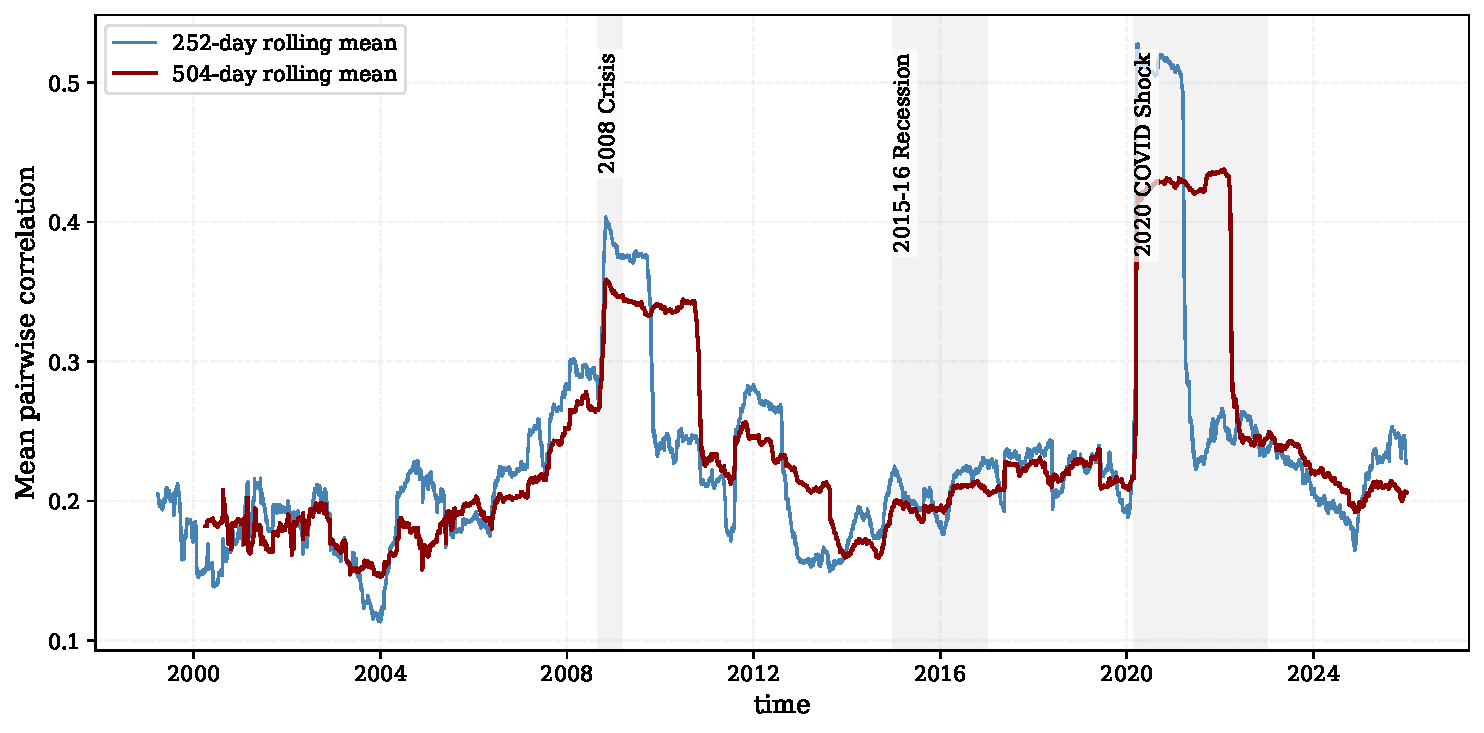
\includegraphics[width=0.9\linewidth]{images/figure_4_rolling_average_correlation.pdf}
\caption{Rolling average market correlation for the core historical universe.}
\label{fig:rolling_corr}
\end{figure}
\FloatBarrier

The rolling average correlation rises during stress periods, including the 2008 global financial crisis, the Brazilian recession period around 2015--2016 and the 2020 COVID shock. These episodes indicate stronger market-wide synchronization. This is precisely the kind of collective behaviour that can dominate the first eigenvalue of the correlation matrix.

Figure~\ref{fig:dynamic_pairwise} adds a more granular view by showing selected pairwise dynamic correlations under different estimators. The objective is not to replace the full matrix but to show that individual dependencies can change substantially over time.

\begin{figure}
\centering
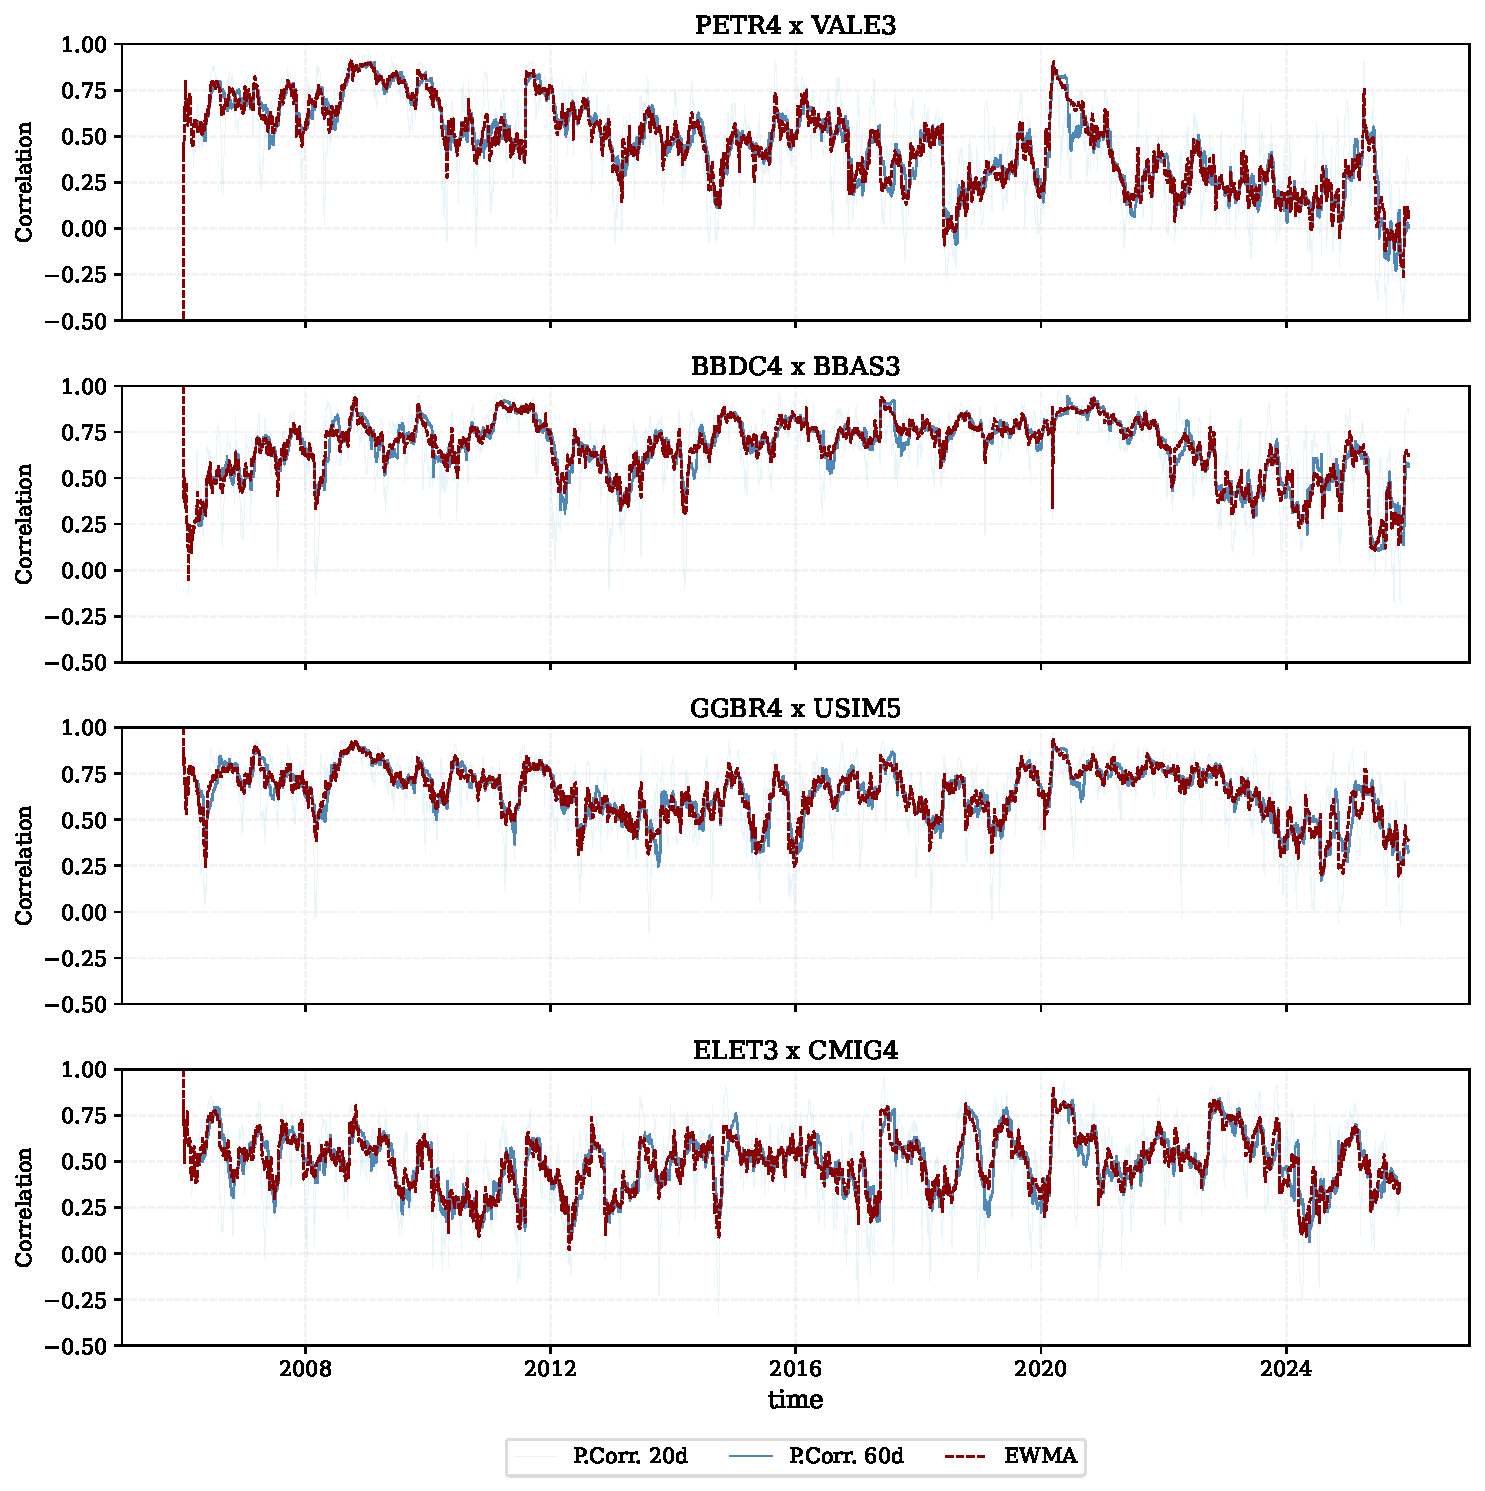
\includegraphics[width=\linewidth]{images/figure_5_dynamic_pairwise_correlations.pdf}
\caption{Dynamic pairwise correlations for selected asset pairs. Short-window, longer-window and EWMA estimates highlight the instability of individual dependencies.}
\label{fig:dynamic_pairwise}
\end{figure}
\FloatBarrier

The dynamic pairwise figure shows why a single full-sample correlation should be interpreted carefully. Short-window correlations react quickly but are noisy; longer-window estimates are smoother but slower; EWMA estimates provide an intermediate view. This motivates the use of RMT and filtered networks as structured summaries of a noisy and time-varying dependency system.
